\PID 
Нека је  
дат систем једначина
$
\displaystyle
\left\lbrace
\begin{array}{l}
\left({\rm D}^2 + \dfrac{1}{25} \right) g(t) = x(t) 
\\[4mm] \displaystyle
y(t) = g(t) \cdot \sum_{k=0}^{\infty} \updelta(t - kT - \uptau)
\end{array} 
\right.,$
где је $T = 10\uppi$, а ${\rm D}$ је оператор 
диференцирања. Дати систем једначина описује
каузалан \textit{LTI} систем чији је једини улаз 
$x(t)$ а једини излаз $y(t)$.
Израчунати \textbf{минималну} вредност параметра $\uptau > 0$ тако да је посматрани систем
стабилан у \textit{BIBO} смислу.
\\[2mm]

\textsc{\underline{Решење}}: Стабилност система испитујемо испитивањем апсолутне интеграбилности импулсног одзива
$\int_{-\infty}^{\infty} |h(t)| \de t < \infty$, дакле за $x(t) = \updelta(t)$. Прво одређујемо одзив $g(t)$ у том случају,
решавањем $\left({\rm D}^2 + \dfrac{1}{25} \right) g(t) = \updelta(t)$, чиме се добија 
$g(t) =  5 \sin\left(\dfrac{t}{5}\right) \uu(t)$, одакле се заменом у израз за $y(t)$ добија импулсни одзив: 
\begin{equation}
    h(t) = 5 \sin\left(\dfrac{t}{5}\right) \uu(t) \cdot \sum_{k=0}^{\infty} \updelta(t - kT - \uptau) 
         = \sum_{k=0}^{\infty}  5 \sin\left(\dfrac{kT + \uptau}{5}\right) \updelta(t - kT - \uptau). \label{eq:\ID.h}
\end{equation}
Услов стабилности се може онда изразити као
\begin{equation}
    \int_{-\infty}^{\infty} |h(t)| \de t = \left| \sum_{k=0}^{\infty}  5 \sin\left(\dfrac{kT + \uptau}{5}\right)\right| < \infty.  
\end{equation}
Једини начин на који је могуће да добијена сума конвергира јесте да је
$\sin\left(\dfrac{kT + \uptau}{5}\right) =  \sin\left(2\uppi k + \dfrac{\uptau}{5}\right) = 0$ за све $k \in \mathbb{N}$,
односно, треба да буде $\dfrac{\uptau}{5} = m\uppi$, где је $m \in \mathbb{Z}$. Коначно, минимално $\uptau>0$ које задовољава наведени
услов јесте $\uptau = 5\uppi$, а минимално позитивно решење је када је $\uptau = 5\uppi$.

\begin{figure}[!b]
    \centering
    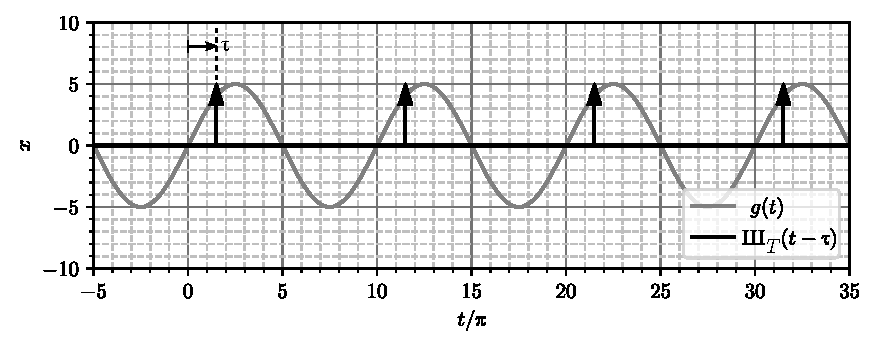
\includegraphics{fig/delta_odabiranje_sin_edit.pdf }
    \caption{}
    \label{fig:\ID.ideja}
\end{figure}

Други део поступка може се размотрити и графички. На слици \ref{fig:\ID.ideja} приказан је одређени импулсни одзив 
$g(t)$. У изразу \eqref{eq:\ID.h} може се препознати други члан као $\III_T(t - \uptau)$, односно, импулсни одзив система
је $h(t) = g(t) \cdot \III_T(t - \uptau)$, што је илустровано на слици \ref{fig:\ID.ideja}. Пошто су периоди функције $g(t)$ и функције
$\III_T(t - \uptau)$ исти, прираштај интеграла $\int_{-\infty}^{\infty} |h(t)| \de t$ је увек исти за сваки делта импулс, 
то значи да ће тај интеграл бити коначан само ако делта импулси „гађају“ нуле функције $g(t)$, што се дешава када је
$\uptau = kT/2 = 5k\uppi$.
